%%%%%%%%%%%%%%%%%%%%%%%%%%%%%%%%%%%%%%%%%%%%%%%%%%
% This latex format is designed by               %
% Quwsar Ohi                                     %
% Intake 33                                      % 
% Department of CSE                              %
% Bangladesh University of Business & Technology %
%%%%%%%%%%%%%%%%%%%%%%%%%%%%%%%%%%%%%%%%%%%%%%%%%%

% Size of character is set to 12pt
\documentclass[12pt]{ucthesis}
\usepackage{url}
\usepackage{microtype}

% Hides "Chapter X" for each chapter
\usepackage{titlesec}
\titleformat{\chapter}[display]
  {\normalfont\bfseries}{}{0pt}{\Large}


% Use if you need landscape figures
%\usepackage{rotating}
\usepackage{lscape}

\usepackage[pdftex]{graphicx}

% For list of symbols and abbreviations
\usepackage[automake, acronym]{glossaries}

%\usepackage[pdftex,
%            plainpages=false,
%            breaklinks=true,
%            colorlinks=false,
%            urlcolor=blue,
%            citecolor=blue,
%            linkcolor=blue,
%            bookmarks=true,
%            bookmarksopen=true,%
%            bookmarksopenlevel=3,
%            pdfstartview=FitV,
%            pdfauthor={Quwsar Ohi},
%            pdftitle={thesis},
%            pdfkeywords={thesis, BUBT},
%            ]{hyperref}


% For \citep and \citet citations
%\usepackage[authoryear,round,longnamesfirst]{natbib}

% Bibliography style
\usepackage[numbers,sort&compress]{natbib}
%\usepackage{natbib}

%\bibliographystyle{abbrv}
%\bibliographystyle{ksfh_nat}
\bibliographystyle{unsrt}
%\bibliographystyle{plainnat}

\def\newblock{\ }

% Only use if graphs are plotted by latex
\usepackage{pgfplots}
%\usepackage{geometry}
% Only use if grantt chart are plotted by latex
\usepackage{pgfgantt}

% Math Symbols
\usepackage{amssymb}
\usepackage{amsmath}
\usepackage{mathtools}
\DeclareMathOperator*{\argmax}{arg\,max}

%\usepackage[overload]{textcase}

% Page margin setup
\usepackage[letterpaper]{geometry}
\setlength{\parindent}{0.25in} \setlength{\parskip}{6pt}
\geometry{verbose,
          nohead,
          tmargin=1.2in,
          bmargin=1in,
          lmargin=2in,
          rmargin=1.2in}

\setcounter{tocdepth}{2}

% Adding symbols and abbreviations from file
\input{symbols}
\input{abbreviations}
\makeglossaries


% -------------------------------------------------------------
% Document start
\begin{document}


% Front Page
% Set Paper Title
\title{A Blockchain Based Secured Land Record System Using Hyperledger Fabric}

% Name and ID of authors
% There are total 6 authors, named as authorA, authorB, to authorF
\authorA{Md. Mahedi Hasan}
\authorAID{17182103278}

\authorB{Md. Hasibur Rahman}
\authorBID{17182103280}

\authorC{Tahmid Ahmed}
\authorCID{17182103311}

\authorD{Md. Aminul Islam}
\authorDID{17182103319}

\authorF{Alhaj Hossen}
\authorFID{17182103335}

% Degree Date
\degreemonth{March} 
\degreeyear{2022}

% Degree and field
\degree{Bachelor of Science}
\field{Computer Science and Engineering}
\campus{Mirpur, Dhaka}

% Defence Date
\defensemonth{March}
\defenseyear{2021}
\numberofmembers{5}


\maketitle

% If committee membership required
%
%\chair{Ernest Merkel, Ph.D.} 
%\chairdesignation{Associate Professor}
%\chairdepartment{Statistics Department}

%\othermemberA{Kathy Abernathy, Ph.D.} 
%\othermemberAdesignation{Associate Professor}
%\othermemberAdepartment{Engineering Department}

%\othermemberB{Peter Chan, Ph.D.}
%\othermemberBdesignation{Associate Professor}
%\othermemberBdepartment{Mathematics Department}


%\othermemberC{Jason Pearson, Ph.D.\\ & Professor \\ & Chemistry Department} 
%\othermemberCdesignation{}
%\othermemberCdepartment{}

% Add Copyright Terms if required
%\copyrightyears{seven}
%
% Add Copyright Page if Required
% \copyrightpage

% Add Committee Membership Page if Required
%\committeemembershippage
%\approvalpage

\begin{frontmatter}



\chapter*{Abstract}
\addcontentsline{toc}{chapter}{Abstract} 
    
    In Bangladesh, scarcity of land and fast population grow this putting a strain on the land-man ratio. The property ownership registration system in Bangladesh is incomplete and insufficient. As a result, various government agencies handle various documents, and bureaucracy flaws enable organized crime. Considering these, we are proposing a method where we have come up with a Blockchain based solution. We build a Blockchain based system to ensure that individuals are not deceived under any circumstances. In our system, where land data will be safe  and  secure,  data  synchronization  and  transparency  will  be  available, as well as ease of access, irreversible record management, and rapid and low cost quick solutions. We designed a modern architecture to digitally store land records using Blockchain based Hyperledger Fabric to ensure land security. This proposed model has been presented by private Blockchain, taking into account the technological expertise and authority of the people and government. Finally, we compare our proposed architecture with the existing land records management model. Our system provides  more  security  and  data  privacy  than  other  models  and  saves both money and time in our daily lives. This will ensure that our system is transparent and acceptable in all directions.

% Declaration
% ----------------------------------------------

\declaration
 

%\restoregeometry 
\chapter*{Acknowledgement}
\addcontentsline{toc}{chapter}{Acknowledgement} 
    We would like to express our heartfelt gratitude to the almighty Allah who offered upon our family and us kind care throughout this journey until the fulfilment of this research.

    Also, we express our sincere respect and gratitude to our supervisor Md. Anwar Hussen Wadud, Assistant Professor, Department of Computer Science and Engineering, Bangladesh University of Business and Technology(BUBT). Without his guidance, this research work would not exist. We are grateful to him for his excellent supervision and for putting his utmost effort into developing this project. We owe him a lot for his assistance, encouragement, and guidance, which has shaped our mentality as a researcher.

    Finally, we are grateful to all our faculty members of the CSE department, BUBT, to make us compatible to complete this research work with the proper guidance and supports throughout the last four years.



%\newgeometry{top=5cm, bottom=10cm}

%\par\vfill\break % Break Last Page
%\advance\vsize by 12cm % Advance page height
%\advance\voffset by -4cm % Shift top margin
\chapter*{Approval}
\vspace{-2mm}
\addcontentsline{toc}{chapter}{Approval}
This report \textbf{“A Blockchain Based Secured Land Record System Using Hyperledger Fabric”} submitted by\textbf{Md. Mahedi Hasan, Md. Hasibur Rahman, Tahmid Ahmed, Md. Aminul Islam, and Alhaj Hossen ID no: 17182103278, 17182103280, 17182103311, 17182103319, and 17182103335} Department of Computer Science and Engineering (CSE), Bangladesh University of Business and Technology (BUBT) under the supervision of \textbf{ Md. Anwar Hussen Wadud, Assistant Professor}, Department of Computer Science and Engineering (CSE) has been accepted as appeasement for the partial fruition of the requirement for the degree of Bachelor of Science (B.Sc.) in Computer Science and Engineering and endorsed as to its contents.
\enlargethispage{1\baselineskip}
\newline
%\newline
%\newline
\begin{tabular}{l}

\hspace{-0.8cm}------------------------- \\
\hspace{-0.8cm}\textbf{Supervisor:}\\
\hspace{-0.8cm}\textbf{Md. Anwar Hussen Wadud}\\
\hspace{-0.8cm}\textbf {Assistant Professor}\\
\hspace{-0.82cm}Department of Computer Science and Engineering (CSE)\\
\hspace{-0.82cm}Bangladesh University of Business and Technology (BUBT)\\
\hspace{-0.82cm}Mirpur-2, Dhaka-1216.\\
\\
\\
\hspace{-0.8cm}--------------------------- \\
\hspace{-0.8cm}\textbf {Md. Saifur Rahman}\\
\hspace{-0.8cm}\textbf{Assistant Professor and Chairman}\\
\hspace{-0.82cm}Department of Computer Science and Engineering (CSE)\\
\hspace{-0.82cm}Bangladesh University of Business and Technology (BUBT)\\
\hspace{-0.82cm}Mirpur-2, Dhaka-1216.\\

       
        \end{tabular}
%\vspace{10mm}

 
%\par\vfill\break % Break the page with different margins
%\advance\vsize by -12cm % Return old margings and page height
%\advance\voffset by 4cm % Return old margings and page height
    
   
 
  % We do hereby acknowledge that the research works presented in this thesis entitled "A Blockchain Based Secured Land Record System Using Hyperledger Fabric" result from the original works carried out by Md. Anwar Hussen Wadud, Assistant Professor, Department of Computer Science and Engineering, Bangladesh University of Business and Technology. We further declare that no part of this thesis has been submitted elsewhere for the requirements of any degree, award or diploma, or any other purposes except for publications. 
   %We further certify that the dissertation meets the requirements and standard for the degree of Doctor of Philosophy in Computer Science and Engineering.
   
   
   




% Some index management
\listoftables
\listoffigures
\listofabbreviations
%\listappendixname

\tableofcontents
\end{frontmatter}
\pagestyle{plain}
\renewcommand{\baselinestretch}{1.66}


% Chapter 1 : Introduction
% -----------------------------------------------
\chapter{Introduction}
\label{introduction}

% Introduction
% -----------------------------------------------
\section{Introduction}
\label{introductionintro}
 Land registration is a system that keeps track of who owns something and what rights they have over it. Blockchain is a remarkable new technology that can provide any agency's systems trust, integrity, and accessibility. A database, or Blockchain, is a sort of digital ledger. In most cases, Blockchain accumulates data in groups, sometimes known as blocks, that contain sets of data. Blocks have specific storage capabilities, and when filled, they are chained onto the previous block, establishing a data chain known as the "Blockchain." All additional information added after that newly added block is compiled into a new block, which is then added to the chain after it is filled\cite{ref15}.

Hyperledger Fabric is a private Blockchain. Businesses can use distributed ledger technology without exposing their data to the public by using a private Blockchain. This website is password-protected. The Blockchain allows only known nodes to participate in the procedure\cite{rf4}.

The primary problem in the current system is that data is dispersed across multiple government institutions that aren't well-synchronized, enabling hacked persons to modify legal papers. A centralized system will be insufficient to cope with the various land titling frauds in this case\cite{rf3}. In this research, we evaluate Bangladesh's present land registration process and propose a new framework based on Blockchain technology to improve transparency and dependability\cite{rf1}.

In the past, there was a manual system for land registration.
At that time we faced many problems. This existing system
takes a long time. On the basis of Bangladesh, there are some
illegal means of registration. However, before this study, no
work has been introduced on the digitization of land registration
using Hyperledger Fabric framework. In this paper we are
going to introduce the digital version of the land registration system where we use a Hyperledger Framework with
Blockchain technology\cite{rf16}.

The present age is the digital and modern age and technological development is increasing day by day. Everything we
need in our daily lives is going digital. As we have analyzed,
people have already been recording land with pen in hand
which is not going to keep pace with the digital age, and
this manual system leaves people facing a lot of harassment.
However, to analyze human demand, we want to develop a
land record system that is easily accessible to the user. This
system is very easy to use for users and it’s very secure for
user information. The study work's overall performance is as follows: 

• We highlight a current challenge in analyzing human demand in the Secured Land Service.

• We propose a secured land registration model using Hyperledger Fabric based Blockchain network.

• We reduce manual involvement by implementing actual property title assignments and ensuring the security of public land data.


% Problem Statement
% -----------------------------------------------
\section{Problem Statement}
\label{problemstatement}
    
Identification:The major goal of this project is to locate the real  owner of the land or a genuine person and then accept the documents for registration.

Transition Process:A registrar charge is required for each and every registration. To accept the registration, the system requires a one-time prepayment. That is why we have developed a secure transaction mechanism.

Consent Principle:To transfer the land to the buyer, the true owner's consent must be obtained through the land register. The main issues identified during this process are:
\begin{itemize}
    \item Identification of the genuine owner.
    \item Availability of digital signatures to all the users/ owners.
\end{itemize}
 

    
% Problem Background
% -----------------------------------------------
\section{Problem Background}
\label{problembackground}
    
    Distributed network implementation in real life is the main challenge for us. 
Because, land registration system we can use two types of data. One of them is 
public and the other one is private data. Public data is available for every user but 
the private data can see only specific users. Such as,Ac land, Surveyor etc.
 
So , Our main goal is to define who sees the public data and who sees the private 
data

% Research Objectives
% -----------------------------------------------
\section{Research Objectives}
\label{researchobjectives}
    
   The objectives of our research work are as follows:
   \begin{itemize}
    	\item Digitalization.
    	\item The security issue is resolved to a great extent. 
    	\item All information about land sell and buy. 
    	\item Using Blockchain shows public or private data in different categories of users.
    \end{itemize}


% Motivations
% -----------------------------------------------
\section{Motivations}
\label{motivations}
    
Blockchain is a method of storing data that makes it impossible to alter, hack or cheat recorded information on the system. Every block on the chain comprises a number of transactions, and whenever a new transaction happens on the Blockchain, a record of that transaction is recorded to the ledgers of all participants. A decentralized database managed by several parties is referred to as Distributed Ledger Technology (DLT). Hyperledger Fabric is designed to serve as a basis for building modular applications and solutions. Hyperledger Fabric is aiming as an establishment for creating applications or solutions with a secluded architecture. Hyperledger Fabric permits components, such as agreement and participation administrations, to be plug-and-play. Its measured and versatile plan fulfills a wide run of industry utilize cases.
Hyperledger Fabric is a permissioned Blockchain network that is created by companies looking to form a consortium. Each Blockchain network member organization is responsible for preparing their peers to join the network.




% Flow of the Research
% -----------------------------------------------
\section{Flow of the Research}
\label{flowoftheresearch}
    
     
    
    \begin{figure}[ht!]
    \begin{center}
        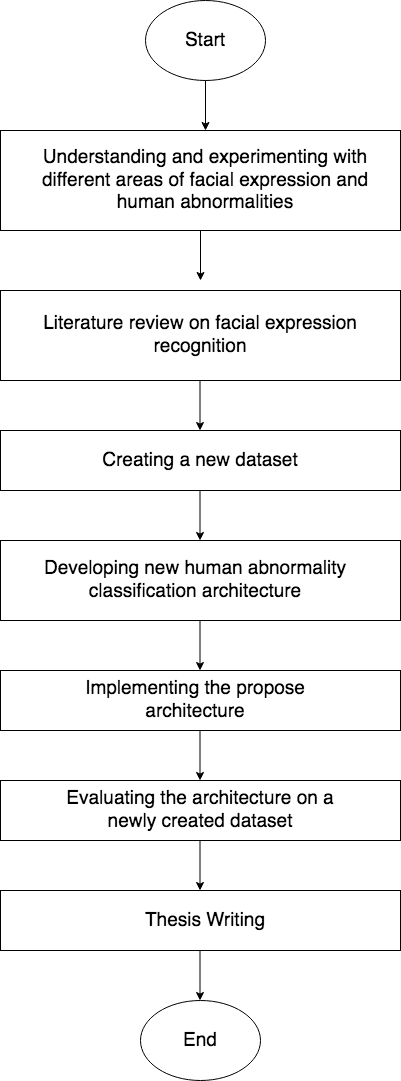
\includegraphics[width=40cm,height=15cm,keepaspectratio]{{./img/flowdiagram.png}}
        %\captionfonts
        \caption[Flow of the work]{The figure illustrates the flow of the thesis work.}
        \label{fig:research_flow}
    \end{center}
    \end{figure}

 
% Significance of the research
% -----------------------------------------------
\section{Significance of the Research}
\label{significanceoftheresearch}
    The digital and contemporary eras are now in full swing. And the pace of technological advancement is quickening. Everything we require in our everyday lives is being converted to digital format. As we've seen, people have been documenting land with a pen in hand for a long time, which will not keep up with the digital era, and this manual approach exposes individuals to a lot of abuse.
However, in order to assess human need, we wish to create a land record system that is user-friendly.Users will find our system to be highly user-friendly, and the information they provide will be kept safe.


% Research contribution
% -----------------------------------------------
\section{Research Contribution}
\label{researchcontribution}
    
    The overall contribution of the research work are:
    
    \begin{itemize}
      
        \item The main contribution of this research is to determine the utilization of the land record system.
        \item In the Secured Land Record System, identifying the current issue in analyzing human demand.
        \item When individuals have the ability to register land, they may assure that no one is hounded by a corrupt individual.
        \item Ensuring that public land information is protected.
    \end{itemize}
    

% Thesis Organization
% -----------------------------------------------
\section{Thesis Organization}
\label{thesisorganization}
    
    The thesis work is organised as follows. Chapter \ref{background} highlights the background and literature review on the field of the Land Verification System. Chapter \ref{existingmodel} contains the existing land verification system in Bangladesh. Chapter \ref{implementation} includes the details of the tests and evaluations performed to evaluate our proposed architecture. Chapter \ref{standardsandchallanges} explains the Standards, Impacts, Ethics, Challenges, the Constraints, Timeline, and Gantt Chart. Finally, Chapter \ref{Conclusion} contains the overall conclusion of our thesis work.
    
% Summary
% -----------------------------------------------
\section{Summary}
\label{introductionsummary}
    
    This chapter provides a comprehensive overview of the problem that our study aim to solve, as well as an explanation of how we accomplished our goals. It also shows the general steps in which we executed our investigation.

% Background
% -----------------------------------------------
\chapter{Background}
\label{background}


% Introduction
% -----------------------------------------------
\section{Introduction}
\label{backgroundintroduction}
    
    There was once a manual method in place for land registration. We had a lot of troubles at this time. This current system takes a long time to finish.
There are some illegal registration methods based in Bangladesh. However, before to this study, no work on the digitalization of land registration utilizing the hyperledger fabric framework has been published.
In this paper, we will present the digital version of the land registration system, which will be implemented using the Hyperledger framework with blockchain technology.

% Literature Review
% -----------------------------------------------
\section{Literature Review}
\label{literaturereview}

Himani Mukne et al. \cite{ref15} paper aims at introducing transparency, especially in the realm of land acquisition and ownership record management. It removes the scope for fraudulence by creating an immutable history of records, which is permanently linked to the system. A peer-to-peer tamper-proof and forge-proof network is leveraged for this purpose, using a permissioned blockchain such as Hyperledger Fabric.

Shariful Islam et al.\cite{rf4} is the underlining technology of Bitcoin. It has been used in many domains such as IoT, healthcare, education, business, Land management and so on. Land Registration and Ownership Management is a very tough process all over the world. This paper proposes a permissioned blockchain-Hyperledger based solution model to solve the problems of land registration and ownership management.

Kazi et al.\cite{rf3} suggested a Hybrid Blockchain-
based system that assures stakeholder coordination, data transparency, ease of
access, and controls immutable transaction records in this research. Given the
government’s and general public’s technological immaturity, they suggested a
three-stage Blockchain adoption strategy that begins with public Blockchain and
progresses to a large-scale full hybrid Blockchain. 


Md Sakibul Islam et al.\cite{rf1} proposed digital land registration model, where they
used Ethereum, a public and permissioned Blockchain to build their model. In
their article, the privacy question is answered to a large extent by integrating the
land registry on Blockchain. This will be the most suited and also give infinite
processing capabilities, but there’s been no earlier work on private Blockchains
such as Hyperledger Fabric

Zhang et al. \cite{rf16} Internet of Energy is a combination of power grid and Internet. Different forms of energy needs to interconvert, so it is necessary to make power trading in this distributed system. Hyperledger-Fabric is the one of typical framework of blockchain, which could provide a platform for distributed ledger. It has distributed blocks and ledgers to make decentralized trading by using blockchain technology for Internet of energy.



Papantoniou et al.\cite{rf2} Due to the complexity of the technology, its maturity level, and unorthodox first usage that does not reveal the true value of blockchain. people have conflicting perspectives and attitudes about blockchain technologies. As previously stated, the initial blockchain implementations were public implementations for cryptocurrencies.

J. Michael et al.\cite{rf7} In the short run, blockchain might cut the time it takes for Torrens jurisdictions to approve new title certificates. In the long term, blockchain registries may be able to benefit from higher liquidity than abstract title jurisdictions, which include the vast majority of U.S. states and counties. The fundamental benefit of the Torrens system is increased title security. A certificate of title is a government-backed promise of ownership that contains all encumbrances listed on the title document. This makes it simpler to transfer ownership safely and can significantly reduce the number of title disputes that burden the judicial system, particularly in areas with inaccurate or missing property records.
 

Sharma et al.\cite{rf6} propose a decentralized private blockchain system with several consensus methods for confirming each land transaction between new and old owners without the participation of third parties.




Thakur et al. \cite{ref_14} in this paper explores the usage of. Blockchain Technology for Land Records Management in India. It highlights issues, such as minimal transparency, accountability and incoherent data sets with different Government. Departments pertaining to the same piece of land. Delays in the current Land Records management process.

Yaga at al.\cite{rf5} Blockchains are tamper evident and tamper resistant digital ledgers. They enable a community of users to record transactions in a shared ledger. Under normal operation of the blockchain network no transaction can be changed once published. This document provides a high-level technical overview of blockchain technology.

 Nasir at al \cite{rf21} Blockchain is a key technology that has the potential to decentralize the way we store, share, and manage information and data. Hyperledger Fabric is an open source, permissioned blockchain that was introduced by IBM. The performance analysis results across all evaluation metrics, scalability, throughput, execution time, and latency.
 
Wadud at al.\cite{refAHW} Patient-centric Agents manage patient's data and coordinate authorization to form a secure channel to transmit data to the private blockchain. Hybrid consensus by combining Proof of Integrity (PoI) and Proof of Validity (PoV) is used to protect data privacy and integrity. Merkle Tree algorithm was used for data processing and authentication when uploading it to a cloud database.

Biswas at al. \cite{biswas2021landchain} The Fourth Industrial Revolution will be solely driven by a set of cutting-edge technologies. Countries who are well prepared and trained to adopt these technologies have a better chance of success. In Bangladesh, the current land registration system has some major drawbacks. We propose a system based on blockchain that have the capability to dramatically reduce the time taken to sell or buy land property.

Mukherjee at al. \cite{mukherjee2020hyper} This paper promises benefits in trustability, collaboration, organization, identification, credibility, and transparency. In this paper, we'll describe about blockchain on E-voting which offers to the electoral process is a combination of accuracy, transparency, and immutability. No matter the arena, voters deserve trust. They demand it, they deserve it.

Al-Amin at al.\cite{al2021towards} In this research paper, we propose an effective, efficient, and satisfactory model or system and service solution to agro traders and also a food traceability system based on blockchain. And through the blockchain, smart contract, and the help of IoT sensors, we tried to do maximum effort to reduce human intervention.

Hossain at al.\cite{9642537} Blockchain technology gives a framework for safe transactions across networks expect to its immutability and unchanging features. This system protects all supplies from fraud and provides a tracking tool to track all previous network activities. Online Medical Record (OMR) system allows patients to share information and control the health status of specific people.

Biswas at al.\cite{biswas2022drlas} The Land Administration System (LAS) is a salient infrastructure. Both the digital (traditional database system) and the manual methods are applied. In this work, the implementation of a blockchain-based system is proposed to build a System for Land Administration. The proposed framework was simulated and showed that the framework contributed to developing an effective system of land administration.

Jobaer at al.\cite{mist2021} Medical data monitoring systems are suffering key challenges in phases of information immutability, traceability, transparency, observation, data validation, access permission, reliability, privacy, and safety. This document suggests a BC framework to efficiently and securely collect and keep health records. It represents a reliable and skilled means of achieving healthcare data for patients, physicians, and security insurance agencies.

Rabbi at al.\cite{rabbi2021bls} Blockchain technology is a decentralized ledger system that records immutable data. This paper focuses on how to make a partially decentralized system that we can use in banking agencies to sanction the loan. The proposed model also uses the Hyperledger Fabric blockchain to implement the smart contracts method called 'chaincodes'.

Ahmed at al.\cite{ahmed2021dbst} Researchers are working towards finding more flexible solutions in case of range queries. In this work, we propose our model DBST, which uses Binary Search Tree techniques to create and maintain the P2P network. Our proposed model is effective for managing multi-attribute range queries and fast searching with cost of O(log n + k).

Akhund at al.\cite{biswas2021biot} The proposed model combines AI, IoT, and Blockchain to develop a smart and futuristic agricultural system. It provides farmers with a secure and open transaction approach to rich, new, and effective decision support. It can specifically create the scope of greater agricultural process productivity and help farmers maximize their benefits.

Shahed at al.\cite{ahamed2021bps} Blockchain's yoke is a blessing. Using blockchain is a very easy way tocomplete a payment without making any mistakes. Hackers will never find a way to do their work in this kind of system. Consumers and vendors can see the whole transaction date, time and everything that they dealt with.


However, all these land registration system techniques can not solve
expressions. This all paper is public base record system there are all data are not saved and not secure.
In this paper, we have discussed how to use hyper Ledger Fabric to solve this issue.

% Problem Analysis
% -----------------------------------------------
\section{Problem Analysis}
\label{problemanalysis}
    When we register land using a block-chain-based land registration, all information is updated, and a signature from a land officer is necessary; but, because land officers are not present, we are unable to obtain signatures. However, officers can utilize our system at any moment and sign this paper online, and our land registration procedure will continue. 

% Summary
% -----------------------------------------------
\section{Summary}
\label{backgroundsummary}
    
    Land for sale or  purchases are sometimes documented in this chapter review. So we'll have to go to the land office and deal with a variety of issues. That is why we have implemented an online registration system based on Blockchain technology. People may register land in our system extremely fast and easily. Land may be promptly registered by updating our system with appropriate information.
    


% Existing Model
% -----------------------------------------------
\chapter{Land Verification Process In Bangladesh}
\label{existingmodel}



% Introduction
% -----------------------------------------------
\section{Introduction}
\label{proposedmodelintroduction}
    
    In this section, We describe all the topic of existing model of land verification system in Bangladesh. Here we show some figures and their problem statements.    
    

%  Existing Methods for registering property in Bangladesh
% -----------------------------------------------
\section{ Existing Methods for registering property in Bangladesh}
\label{registeringproperty}

    In Bangladesh, anybody has the legal right to process an immovable property of land. The general public in Bangladesh is ignorant of the complex Record of Rights (ROR) transfer processes, which require hundreds of papers handled by several government departments and take a long time to complete. As a result, intermediaries use every administrative and legal gap they can find and use bribes to alter papers in order to harass ordinary people. This, in turn, generates years of legal wrangling and is the primary source of civil disputes in Bangladesh\cite{rf3}. In Fig.\ref{fig1}, we discussed the current working procedure of the land record management system in Bangladesh.
    
\begin{figure}[!h]
 \centering
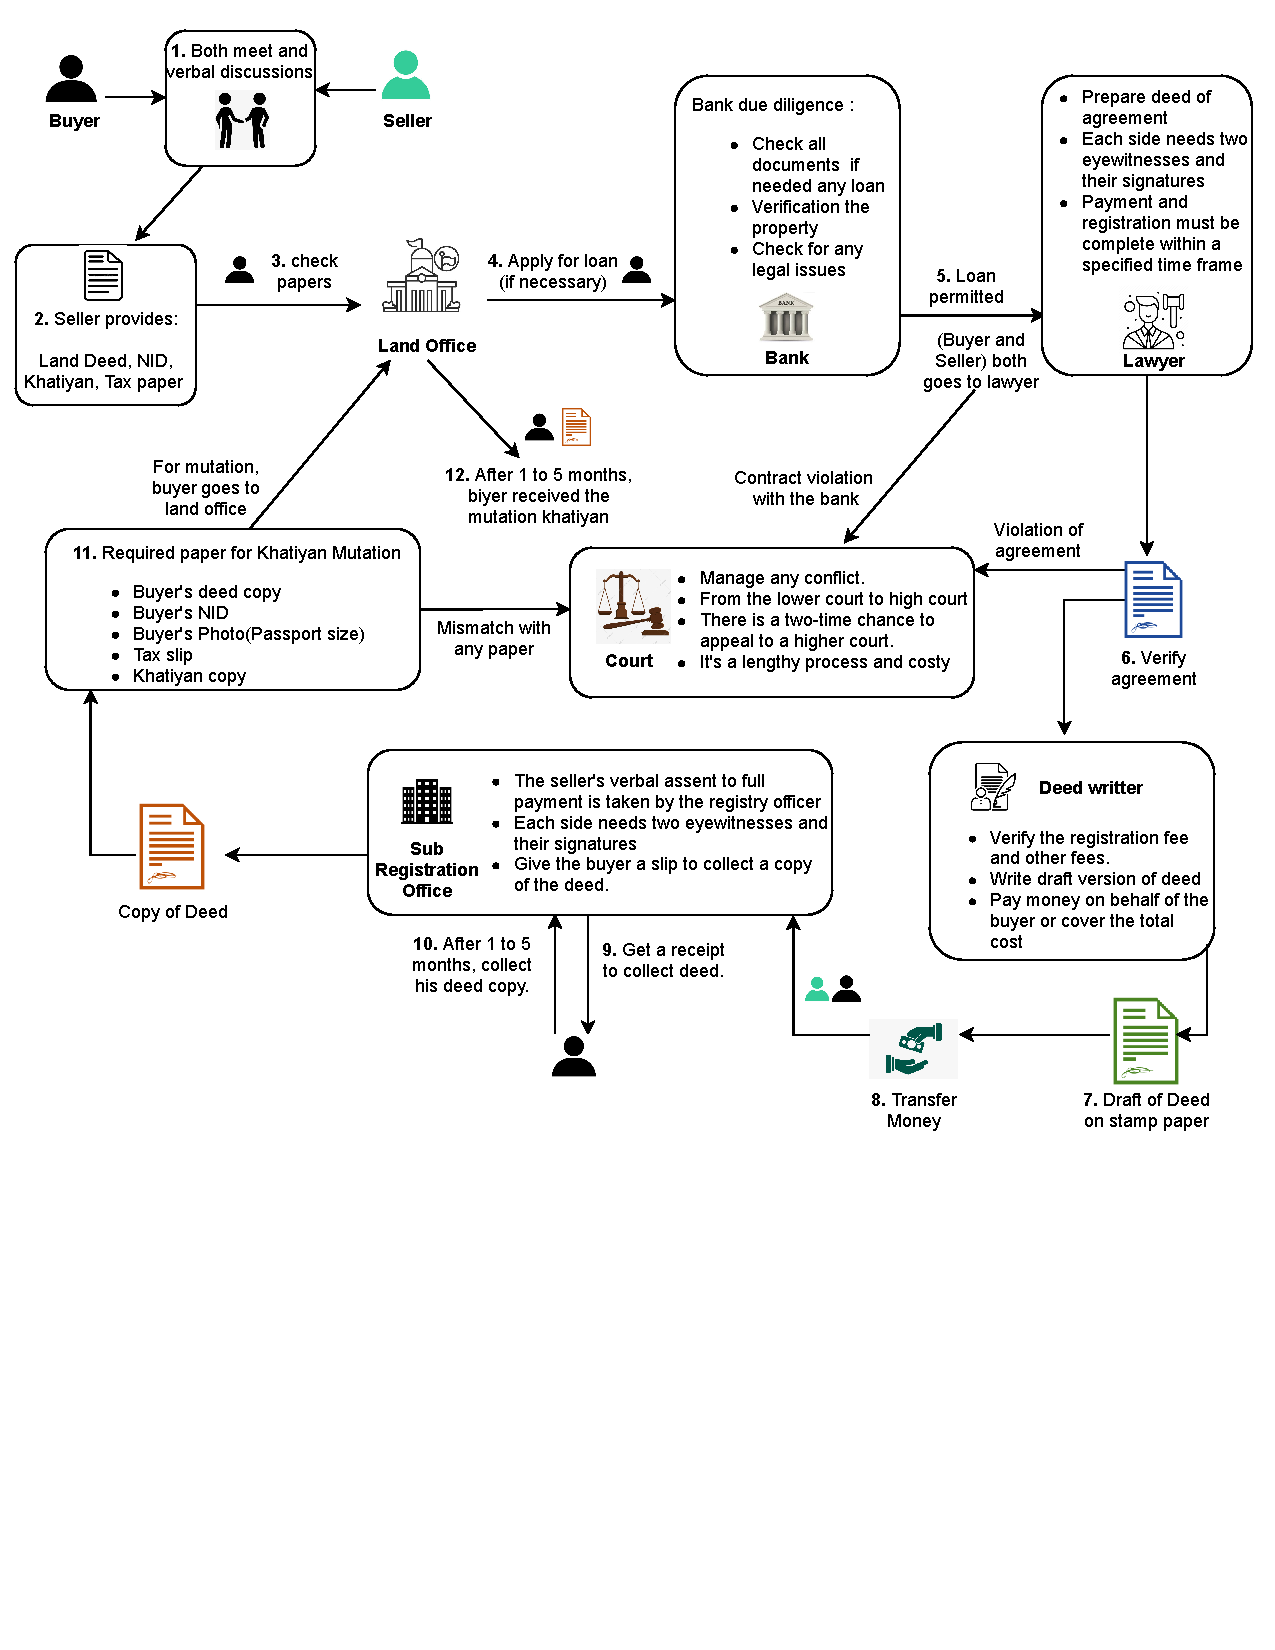
\includegraphics[width=15cm,height=18cm]{{./img/Fig01380.pdf}}
\caption{\textcolor{black}{Existing Methods for registering property in Bangladesh}} 
\label{fig1}
\vspace{-2mm}
\end{figure}
First of all, meet both the buyer and the seller for oral discussions. Then the land documents are examined and verified. The buyer and seller "Agreement to Sell" and get it notarized. If the needed buyer wants to loan for land. Buyer and seller go to a lawyer then verify their agreement. By the lawyer, the document with land money has to be recorded within the stamp paper. Buyer transfer money through the sub-registration office to the seller.  Buyer transfer money through the sub-registration office to the seller. The sub-registration office provides a money receipt to the buyer.  
After one to five months, he collected copies of the documents from the sub-registration office. After obtaining all information, the sub-register office sends it to the land office for mutation purposes. And after one to five months buyer receive the mutation khatiyan through the land office. This is how the existing system works.


% existing verification
% -----------------------------------------------
\section{How to verify if a property is presently owned in Bangladesh?}
\label{existingverification}
    
   Property ownership disputes are quite prevalent in Bangladesh. Property documents are readily faked and untrustworthy. If a person is not careful while purchasing a property, he or she may encounter issues, including a possible dispute with the property's ownership at a later date. Verifying land ownership in Bangladesh, on the other hand, is a time-consuming task. A buyer can check the ownership of a property by following the procedures outlined in Fig.\ref{fig2}.
\begin{figure}[!h]
\centering
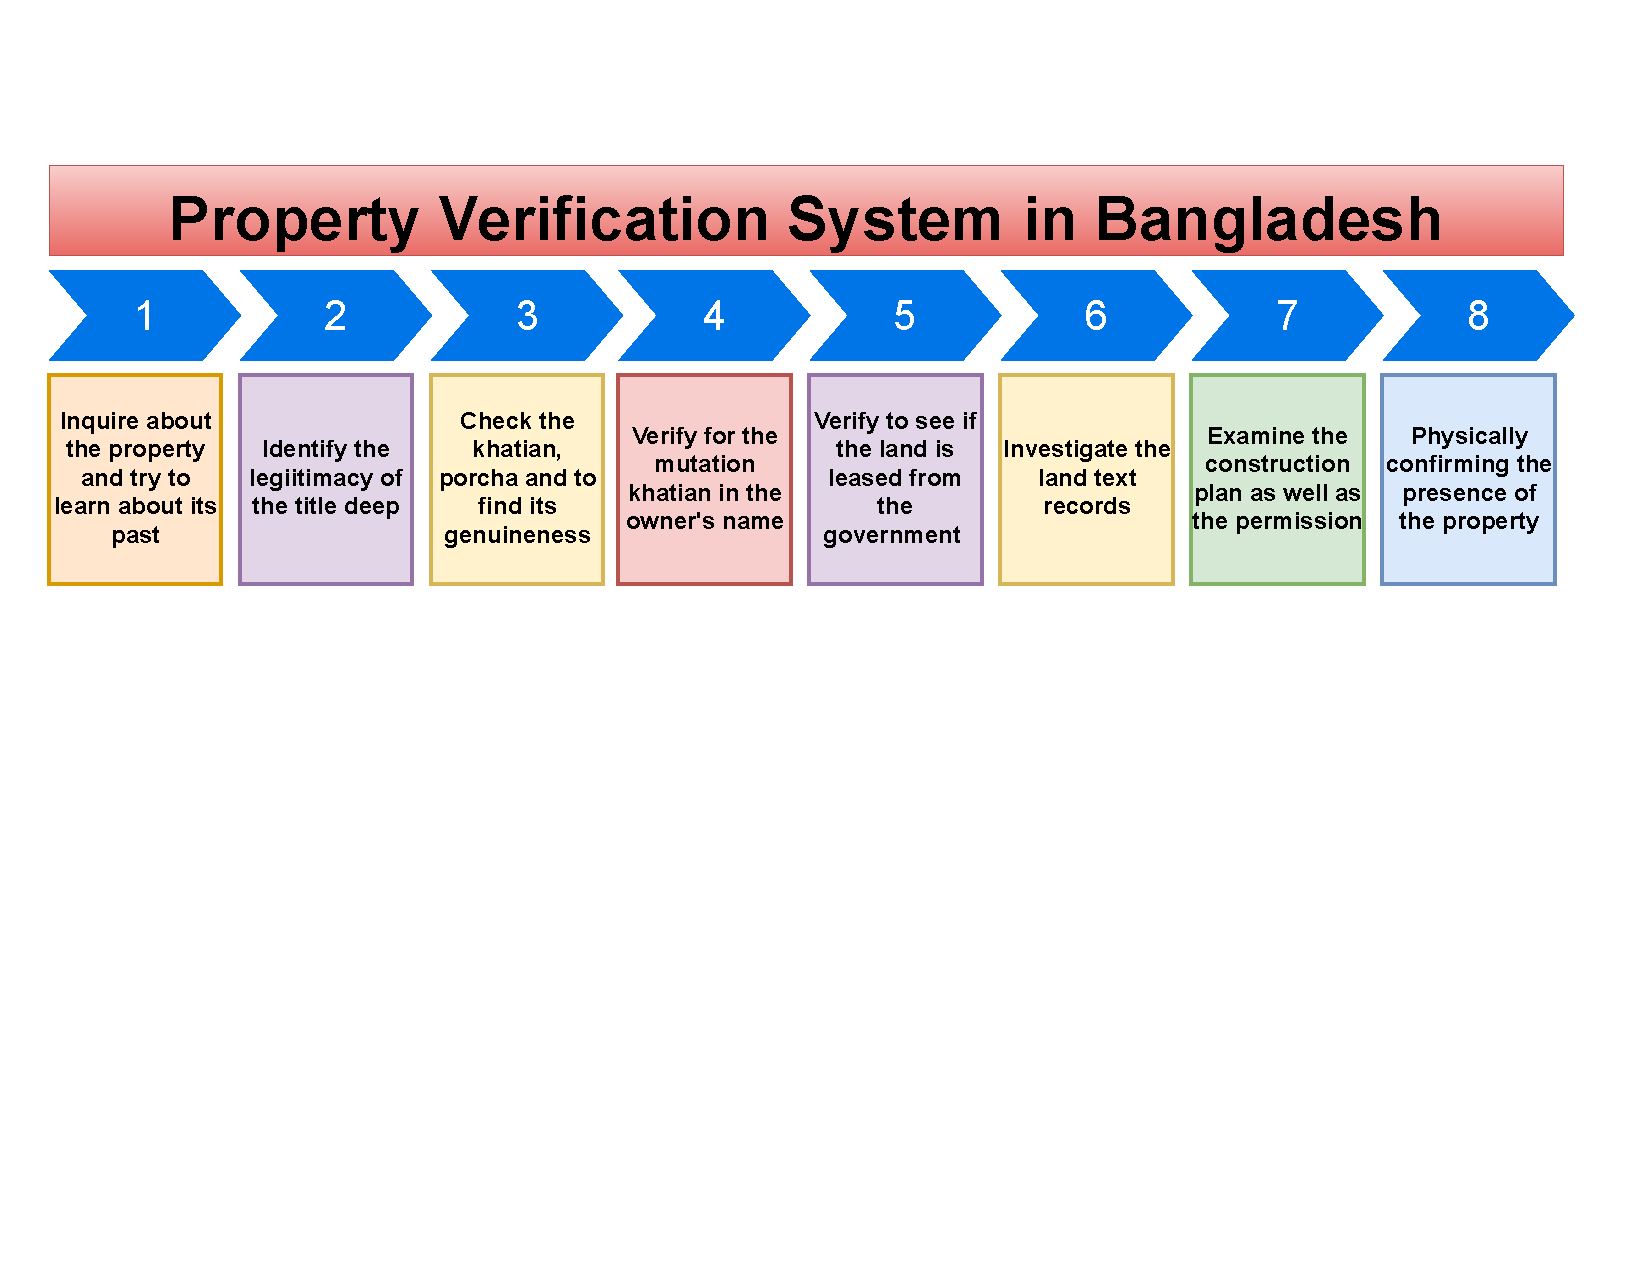
\includegraphics[width=15cm,height=15cm]{{./img/Fig02380.pdf}}
\caption{\textcolor{black}{Property verification system in Bangladesh}} 
\label{fig2}
\vspace{-2mm}
\end{figure}
 


% Complication 
% -----------------------------------------------
\section{Complications with the Present Land Registration System}
 

  There are several problems in our current system.
\begin{itemize}
 \item  \textbf{Verification of Ownership:} Land registration agencies across the world confront a number of problems, one of which is ensuring owner validation.
\item  \textbf{Historical record of Ownership:} These assets do not have a recorded owning history in many cases. When negotiating with unknown persons, getting access to an asset's entire Historical record of Owning (for example, a piece of land) enhances confidence.
\item  \textbf{Illegally Obtained Land Sales:}
Property may be sold without the owners' or insurers' permission, resulting in economic loss.
\item  \textbf{Getting Late For Ownership Of Land Registration:}
Land registration and Postpones in the Transfer of Owning on paper are time-consuming, lasting over the month. Erroneous property value might result in erroneous tax or insurance  premiums.
\item  \textbf{Fails To Recognize a Fraud:}  Present paper-based or technological records are ineffective in preventing identification fraud and identity theft, which can lead to unlawful transactions.
\end{itemize}
    
\section{Related Works}

Md Sakibul Islam et al.\cite{rf1} proposed digital land registration model, where they used Ethereum, a public and permissioned Blockchain to build their model. In their article, the privacy question is answered to a large extent by integrating the land registry on Blockchain. This will be the most suited and also give infinite processing capabilities, but there's been no earlier work on private Blockchains such as Hyperledger Fabric.
%\vspace{2mm}
Due to the complexity of the technology, its maturity level, and unusual first implementation that does not emphasize the true benefit of Blockchain, consumers have diverse opinions and attitudes about the technology \cite{rf2}. They explained the earliest Blockchain technologies were public implementations for cryptocurrencies.
%\vspace{2mm}
Kazi et al.\cite{rf3} suggested a Hybrid Blockchain-based system that assures stakeholder coordination, data transparency, ease of access, and controls immutable transaction records in this research. Given the government's and general public's technological immaturity, they suggested a three-stage Blockchain adoption strategy that begins with public Blockchain and progresses to a large-scale full hybrid Blockchain. To establish an unchangeable and genuine database for land purchasers and owners, certificates were specially formatted and encrypted on the public Bitcoin Blockchain \cite{rf5}.
%\vspace{2mm}
The system proposed in \cite{rf6} this paper follows a decentralized approach of private Blockchain with various consensus algorithms for validating each transaction of land between the new owner and old owner without the involvement of third parties.
%\vspace{2mm}
For a safe and trustworthy land register system, a Blockchain-based architecture is being developed by using ethereum \cite{rf7}. 
Table \ref{tab1} shows the recent works of the different proposed models with our proposed model. Mukne et al.\cite{ref15} propose a single-level anti-corruption model where anyone can access the system with admin permission. This model enables internet protocol  Edge Services (IPES). Consider column two Alam et al.\cite{rf3}, proposes a Three-phase Digitized model where anyone can access it easily. This model enables internet protocol  Edge Services (IPES). Consider column three Thakur et al.\cite{ref11}, proposes a single phase Ownership Transparent model where anyone can't access the system because of the private data. This model disables the internet protocol  Edge Services (IPES). Consider our proposed model as an Archive digitization model where anyone can access the system with admin permission. This model enables internet protocol  Edge Services (IPES).
\begin{table}[!t]
\caption{Compression of Different Proposed Model }
\label{tab1}
 
\scalebox{0.6}{
\begin{tabular}{|l|l|l|l|l|}

\hline
Keyword &  Mukne et al.\cite{ref15} & Alam et al.\cite{rf3} & Thakur el al.\cite{ref11} & Our Proposed Model\\
\hline
Propose year & (2019) & (2020) & (2019) & (2021)\\
Country &  India & Bangladesh & India & Bangladesh\\
Challenge & Anti-corruption & Digitized & Ownership Transparent & Archive digitization\\
Proposed model & One phase & Three phase & One phase & Incremental two phase\\
Blockchain \hfill \break
Architecture & Permissioned & Public and hybrid & Privet or Public & Permission\\
IPES & Enabled & Enabled & N/A & Enabled\\
Experimental Result & Moves phase One to two & Prototype & N/A & Compared with benchmark\\
\hline

\end{tabular}}
 
\vspace{-4mm}
\end{table}
	 
% Summary
% -----------------------------------------------
\section{Summary}
\label{modelsummary}
    
    This section covers the existing land record system's design and categorization process. The main design is built on a combination of convolutional Blockchain and land data.




% Implementation, Testing and Results Analysis
% -----------------------------------------------
\chapter{Proposed Model, Testing, and Experimental Analysis}
\label{implementation}


% Implementation, Testing and Results Analysis
% -----------------------------------------------
\section{Introduction}
\label{implementationintroduction}
    
    This section explains our proposed model workflow. Overall, this section describe how to work our Blockchain based hyperledger fabric land record system model. 

 

\section{Proposed Model Workflow}
%\label{systemsetup}
    
    Distributed network implementation in real life is the main challenge for us. Because land registration system we can use two types of data. One of them is public and the other one
is private data \cite{rf21}. Public data is available for every user but private data can see only specific users. Such as Ac land, Surveyor, etc. So, Our main goal is to define who sees the
public data and who sees the private data. Fig. \ref{fig3} shows the system architecture of the proposed model. When a user comes to take our service, we will first ask him/her to register. If he/she has registered earlier, he/she will need to log in and enter our system. After the login, an option will come in front of him/her by going to the option called Check Details and he/she will have to be given details input of the land which he/she is willing to purchase. As soon as he/she inputs, our system will show him/her all the details of the land where the area, quantity, landowner, and everything will be there. This will prevent the sale of fake land. If all the information is correct, an option will be shown
that says ”Wants to registration”. Clicking on this option will require filling up a form that will provide all rules and conditions and land information, land price, etc. After submitting this form a confirmation letter will go to the landowner. If the owner accepts the form then show the button which is ”pay the registration fee” otherwise there show a massage which is the owner not accepting your request. When paying the registration fee then it transfers to the admin panel where all admin checks the papers. If all papers are well decorated as per the rules and regulations then it’s asking for the payment for land price. The transaction will be credited to Bangladesh Bank. This money will be handed over to the land owner after a certain period of time. Through this, we will also be able to ensure the security of payments. After transaction, a confirmation message would send both the new owner and the old owner. Finally, the new owner will be allowed to download an online copy of the registration along with the government seal.This is how the system works.
\vspace{-2mm}
 \begin{figure}[!t]
 \centering
\includegraphics[width=18cm, height=20cm]{./img/fig03380.pdf}
\caption{\textcolor{black}{Proposed System Framework for Land Registration System}} \label{fig3}
\end{figure}
\vspace{2mm}
    
	 
% System Setup
% ----------------------------------------------- 
\section{Working Strategy of Blockchain Technology}
%\label{systemsetup}
    Blockchain is a decentralized digitized ledger of transactions that is copied and distributed throughout Blockchain's whole computer network structures\cite{refAHW,biswas2021landchain,mukherjee2020hyper,al2021towards,9642537,biswas2022drlas,mist2021,rabbi2021bls,sticounterfeit2021,ahmed2021dbst,biswas2021biot,ahamed2021bps}. Every block of the chain comprises a number of transactions, and when a new transaction takes place on the Blockchain, a record of that transaction is recorded to each user's ledger\cite{rf7}. Blockchain is a distributed ledger system in which data is stored using a hash, which is a cryptographic signature that cannot be changed \cite{rf17}. If hackers wanted to harm a Blockchain system, they'd have to change each block in the chain across all distributed versions.
%\vspace{-2mm}
\subsection{Smart Contract:}
A smart contract is a type of code (written in Go, node.js, or Java) that enforces contract processing between parties using Hyperledger Fabric. Chaincode is a ready-to-install smart contract code bundle. A smart contract is included within a chaincode package. 
Smart contracts use data from the Blockchain to automate corporate processes and workflows\cite{rf18}. The majority of smart contract automation is built in such a way that if anything happens, it will automatically trigger another action that will be posted to the 
ledger. An idea of smart contract automation is monitoring an SLA and subsequently committing a reduction to the ledger for the given IT solution if it is violated. A different example is how, when all the ballots are tabulated, a consensus mechanism immediately commits a winners to the ledger.  

\subsection{Hyperledger Fabric:}
 Hyperledger Fabric is a private
Blockchain. A private Blockchain enables businesses to use distributed ledger technology without providing their data to the public. This is a permissioned Blockchain, which means that only recognized nodes can join the network\cite{rf4}. Its Blockchain may
be observed as a supplementary Blockchain protection system, as people manage an access handle panel to support specific operations to be executed individually by several identifiable members.
The Fabric has several components. The major components of fabric are listed below.
 
\begin{enumerate}
 \item  \textbf{Membership Service Provider(MSP):} Membership Service Provider (MSP) is a component that attempts to encapsulate the membership operation architecture. MSP component that provides the rules for validating, authenticating,and granting network access to identities. MSP works to manage user IDs and ensure authentication to clients who want to join the network and also meantime the client has credentials for transactions. Certificate Authority (CA) and Public Key Infrastructure (PKI) are in charge of ensuring that participants identities are protected (PKI). The MSP makes utilize of a Certificate Specialist, which could be a plug-gable interface that confirms and disavows client certificates upon affirmed character. The Fabric-CA API is the default interface for the MSP[13].Organizations, on the other hand, can use whatever External Certificate Authority they want. Each organization will be responsible for its own MSP. As a result, several MSPs may govern a single Hyperledger Fabric network, with each company bringing its own preference. There are two types of membership service provider. The first one is Local membership service provider. Which is defines user and nodes. It’s define the rights of level. And the another is Channer membership service provider. Which defines administrative and participatory channel level.
 
 \item  \textbf{Client:}
 Clients are apps that suggest transactions over the network on behalf of a user. To connect with a network, the client employs a Fabric SDK. To Understand content in a Fabric Blockchain and an instate Database, the client connect with the SDK. Also the CA authorities also issues a certificate to the client in order to ensure that a legitimate client has begun the network transaction. 
 
  \item  \textbf{Peer:}
 The state and the ledger transact a node to maintain a copy. The ordering service sends blocks to a peer, who maintains the state and ledger. Peers can also serve as special endorsers[14]. An endorsing peer’s unique purpose is to endorse a transaction before it is committed with respect to a specific chaincode. There are different type of peer: Endorsing Peer, Committing Peer, Anchor Peer, Leading Peer. 
 \item  \textbf{Ordering Service:}
 The ordered service offers orderers a connection that
 ensures delivery for the Hyperledger Fabric. Within the requesting stage, the or-derer hubs approve the exchanges against their individual underwriting arrangements. Another step is to concur on the requesting of the transactions concurring to the requesting components put input which can be – to be specific SOLO, Kafka, and Pontoon[15]. The ordering service offers a common communications network between clients and peers, as well as a broadcast service for messages carrying transactional information. The orderers at that point group numerous exchanges into blocks and these blocks are broadcasted to the approving peers.
 \vspace{-4mm}
\end{enumerate}
 \begin{figure}[!t]
 \centering
\includegraphics[width=15cm,scale=0.6]{./img/fig04380.pdf}
\caption{A Hyperledger Fabric Workflow}
\label{fig4}
\end{figure}
\vspace{-2mm}

\subsection{Hyperledger  Fabric  Work  Flow:}
Hyperledger Fabric is a permissioned Blockchain network created by organizations that want to form a consortium. Each Blockchain network member organization is responsible for ensuring that its peers are ready to join the network. Fig. \ref{fig4}  shows the step by step workflow of the Hyperledger Fabric network.

\begin{itemize}
    
\item  A transaction request is initiated by a participant in the member Organization using the client application.

\item The transaction invocation request is broadcast by the client application to the Endorser peer.

\item To confirm the transaction, the Endorser peer examines the Certificate information and the others. The Chaincode (i.e. Smart Contract) is then executed, and the Endorsement replies are returned to the Client. As part of the endorsement response, the endorser peer provides transaction approval or rejection.

\item The client now transmits the authorized transaction to the Orderer peer, who will organize it correctly and put it in a block.

\item The transaction is placed in a block by the Orderer node, then sends the block to the Anchor nodes of the Hyperledger Fabric network's various member Organizations.

\item Anchor nodes then disseminate the block to the rest of their organization's peers. The newest block is then updated in each peer's local ledger. As a result, the ledger is synchronized throughout the whole network. \end{itemize}

% Evaluation
% ----------------------------------------------- 
\section{The Implementation of Blockchain In
Land Registration System}
%\label{evaluation}

    Represents the class diagram of the private Blockchain platform's smart contract development objects (user profile, add a property, transfer property,  user Owned land, transaction) as shown in Fig. \ref{fig5}. Personal information, addresses are stored in the user's NID. With this NID user information, there is an interface for retrieving currently owned land and whether the user exists. A unique ID will be provided to someone while adding the land details to the database. ID ensures ownership of land. The landowner can promote his own land with the unique ID mentioned. when anyone can buy and sell any land or property then can use transfer property and transaction section otherwise he will not use this system.
user owner land section confirms the existence of the landowner and provides information. Similarly, there are necessary identifier information, multiple ownership support, ownership transfer process. On the other hand, a land registration ensures the location of the object and the identifier information. Each object is bound to the user of the Blockchain.
\begin{figure}[!t]
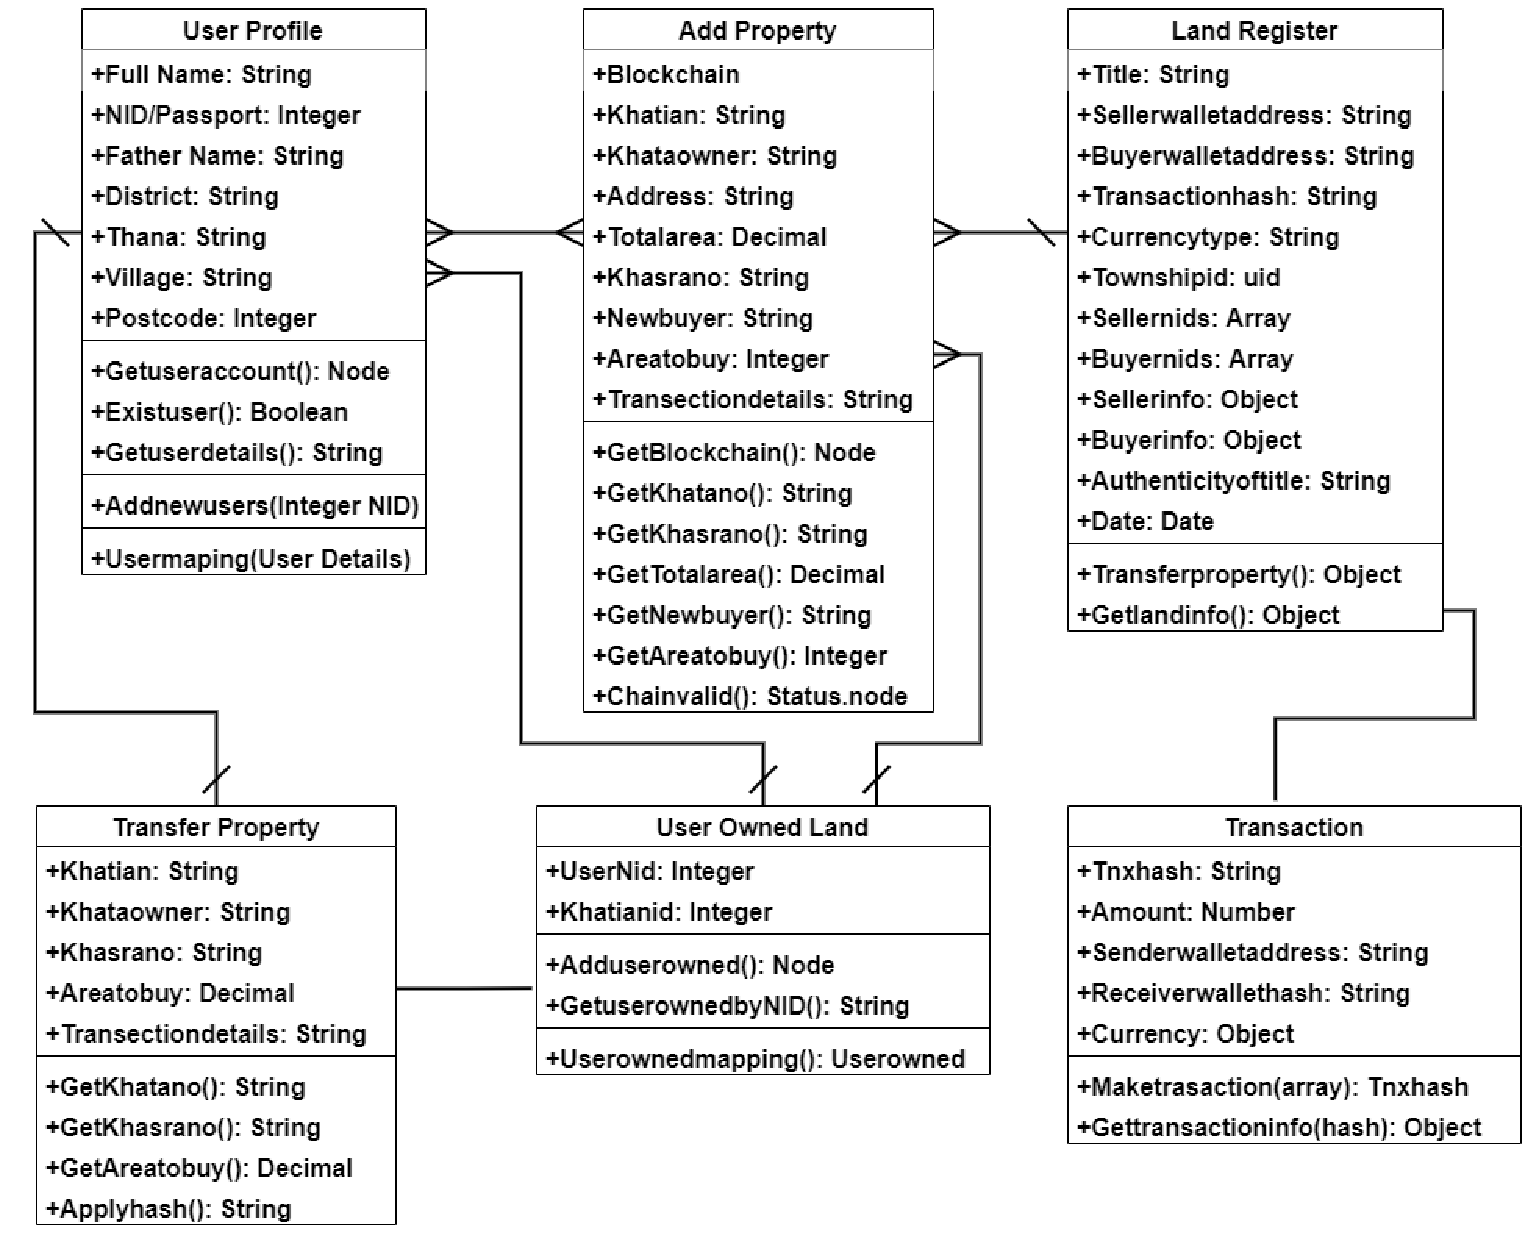
\includegraphics[width=15cm,height=12cm]{img/fig05380.pdf}
\caption{Class Diagram of Development Land Registration System} 
\label{fig5}
\end{figure}
% Results and Discussion
% -----------------------------------------------
\section{ Experimental Analysis}
%\label{resultsanddiscussion}
    \textcolor{black}{In this part, we discuss the proposed system's implementation. There are two types of Blockchain technology, as previously stated: public Blockchain and private Blockchain. We have chosen the private Blockchain for implementation of the proposed system because our proposed system only requires a few nodes and so it is a cost-effective approach. In this paper, a variety of Blockchain implementations have been deployed for constructing Blockchain-based applications \cite{refAHW,biswas2021landchain,mukherjee2020hyper,al2021towards,9642537,biswas2022drlas,mist2021,rabbi2021bls,sticounterfeit2021,ahmed2021dbst,biswas2021biot,ahamed2021bps}. We utilized the Hyperledger Fabric Framework (Linux Foundation, Hyperledger Fabric 3) for Ubuntu (Linux version) to develop the suggested system since it is a private Blockchain implementation with good reliability and a stable community.
We also utilized a Hyperledger Composer that appears to support the Hyperledger Fabric framework and runtime (Linux Foundation, Hyperledger Composer 4). It's a suite of tools for creating Blockchain-based solutions quickly. Other tools used to implement the proposed system involve:(a) Client URL (a library for sending data using different protocols), (b) Docker and docker-compose (used to construct and operate numerous Blockchain network containers), (c) PHP,(Hypertext Preprocessor ), and (d) NodeJs (used to create smart contracts).
 }

\begin{table}[t!]
\caption{System Environment}
\centering
\begin{tabular}{|l|l|}
\hline
\multicolumn{1}{|c|}{{  Hardware}} & \multicolumn{1}{|c|}{{  Configuration}} \\ \hline
{  Operating System}             & {  Ubuntu Linux 18.04.1 LTS}          \\
{  CPU}                & {  Single vCPU @ 2.00GHz} \\
{  Memory}             & {  32GB}                  \\
{  Hyperledger Fabric} & {  Version 1.2}           \\
{  Docker-Compose}     & {  Version 1.5.2}         \\
{  Oracle VirtualBox}  & {  Version 6.1.22}        \\
{  Docker}             & {  Version 1.2.1}         \\ \hline
\end{tabular}
\label{tab2}
\vspace{-2mm}
\end{table}

We perform the offered model utilizing  Hyperledger Composer and Fabric. Through our analyses, we assume that the user data is recovered of the JSON, and demanded data by using the Rest User, for instance, Postman server. Each server was created on the Virtual EC2 instance On AWS, which serves as Ubuntu Linux 18.04.1, 32 GB RAM and single VCPU @ 2.00 GHz on the similarly local PC. As the description of the summary in Table \ref{tab2}. To develop the entire architecture, we applied the Hyperledger composer playground. We utilized Hyperledger Fabric (v 1.2) Linux foundation with hosted an open-source project.


\begin{table*}[t!]
\centering

\caption{Comparison of Existing Works with Proposed Work}
\label{tab3}
%\begin{adjustbox}

\scalebox{0.9}{
\begin{tabular}{|l|c|c|c|c|}
\hline
Key Terms & Mukne et al.\cite{ref_15}          & Alam et al.\cite{rf3}       & Thakur et al.\cite{ref_11}  & Proposed Model          \\ \hline 
User Validation           & \checkmark          & \checkmark         & \checkmark & \checkmark         \\ \hline

Identity Management        & \checkmark         & \textbf{X}          & \checkmark          & \checkmark       \\ \hline

Data Monitoring & \checkmark          & \checkmark          & \checkmark        &\checkmark     \\ \hline


Decentralized Access          & \checkmark        & \checkmark         & \checkmark          & \checkmark        \\ \hline

Availability          & \checkmark         & \textbf{X}        & \textbf{X}       & \checkmark          \\ \hline


Flexibility & \textbf{X} & \textbf{X} & \textbf{X} & \textbf{\checkmark}  \\ \hline
\end{tabular}}
%\end{adjustbox}
\vspace{2mm}
\end{table*}
We have used Blockchain technology to ensure user validation used in our project where each customer ensures validation by matching the land ledger number is shown Table \ref{tab3}. \textcolor{black}{ Identity Management, Data Monitoring and Availability, as well as Decentralized Access, Flexibility and speedy and low-cost quick solutions, will all be accessible in our system, which will keep land data safe and secure.} Our proposed system has a decentralized network with an immutable transaction history for a forge-proof system that can also keep track of all papers online.
\begin{figure}[!t]
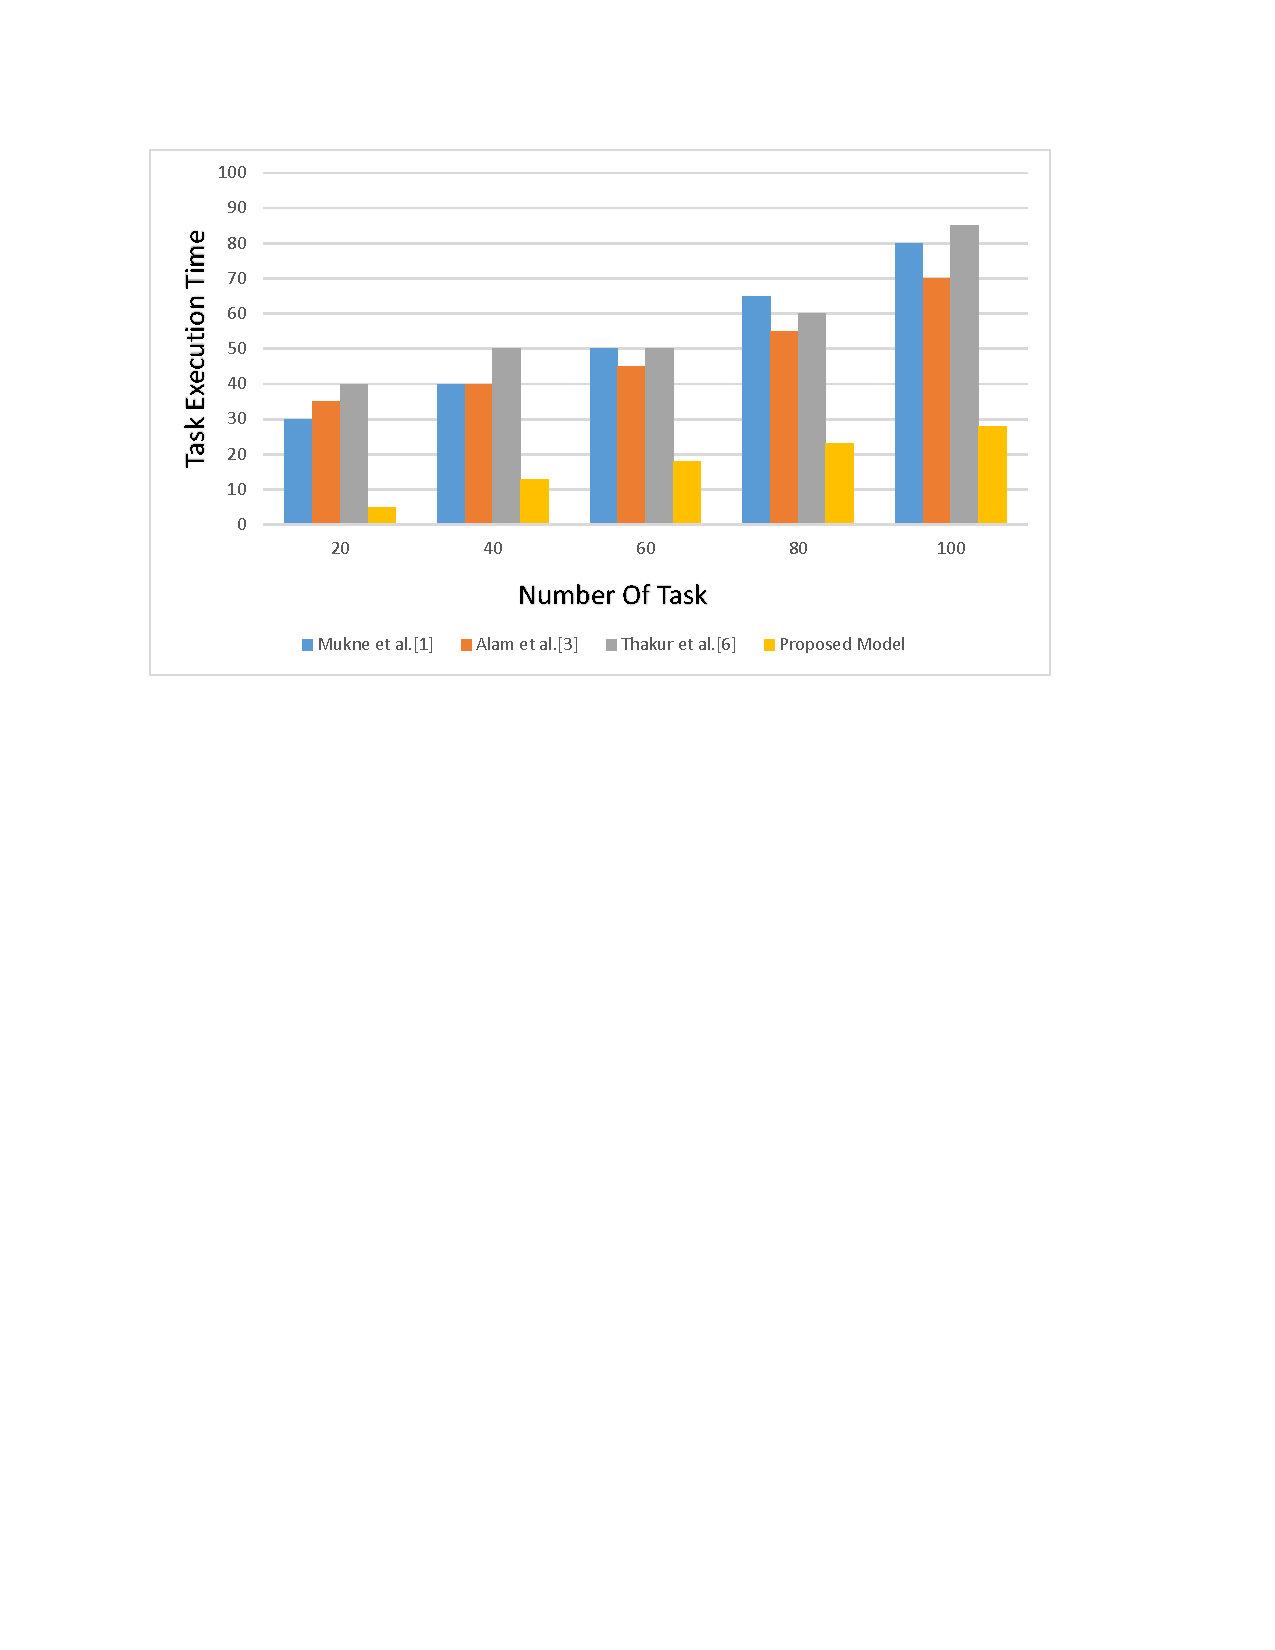
\includegraphics[width=15cm,scale=0.5]{img/Fig06380.pdf}
\caption{\textcolor{black}{Tasks Number vs Execution Time }} 
\label{fig6}
\end{figure}
\textcolor{black}{Lastly, our best reason for all models is the time factor. Other models need maximum time whereas our model takes less time for each task. Additional transactions can be done through our model in the short term. As we see, the graph of Fig.\ref{fig6} shows that each set needs less time to complete the task. But as the number of tasks increases, the number of executions will also increase. Although our model always needs less time than others. When the number of tasks is 0-20 then our model completes the transaction in 5 seconds. Whereas other models require 30-45 seconds. Similarly, when the number of tasks is 20-40, 40-60, 60-80, and 80-100, our model takes 13,18,23,28 seconds respectively whereas other models take up to 40-85 seconds.}

\vspace{-2mm}

% Summary
% -----------------------------------------------
\section{Summary}
%\label{implementationsummary}
    This section explains the architecture of the proposed land record System and classification method. The overall architecture uses the combined convolution Blockchain based and data of land approach.
    
 

% Standards, Impacts, Ethics, and Challenges
% -----------------------------------------------
\chapter{Standards, Constraints, Milestones}
\label{standardsandchallanges}

This segment highlights the thesis work's Standards,  Sustainability, Impacts, and Ethics. Finally, the planned work's Schedules, Tasks, and Milestones are shown.
% Sustainability
% -----------------------------------------------
\section{Standards}
\label{Sustainability}
The Organization For Standardization (ISO) is an independent , non-governmental organization whose members are national standards bodies. It is the biggest creator of voluntary international standards in the world, facilitating global trade by establishing common norms across states. Over 20,000 standards have been established, including everything from manufactured goods and technology to food safety, farming, and wellness. 

ISO 27001 is a set of Blockchain and distributed ledger technology (DLT) standards being developed by the International Standards Organization (ISO). ISO is a non-governmental organization whose members are recognized standards authority who each represent a nation. ISO 27001 is an international standard for information security management. It outlines the standards for creating, deploying, sustaining, and continuously upgrading an information security management system (ISMS), with the goal of assisting companies in securing their data assets.

\section{Sustainability}

Any long-term land management strategy must consider both local needs and economic development prospects. It's easy to use, so communities can take care of basic land administration on their own. The system is low-cost, easy-to-use, and repeatable as compared to traditional registry solutions, and if implemented, it should significantly reduce unit costs for increased volumes of transactions over time. It functions like any other program and appears to the user as such.

In rural locations, a low-cost local register based on the TRUST model can supplement registration efforts by ensuring that registration costs are maintained and benefits are realized.

% Impacts on Society
% -----------------------------------------------
\section{Impacts (on Society)}
\label{impacts}
    
This project will have a very good and effective impact on our society. There is good security in our system as you can easily register land. A person can easily log into our system and buy or sell his land. There will be no need for a third party, and there would be no risk of crime as a result of it.  All the data on this land will go to our central system. In this way, the data will be together, not scattered. Data can be easily found. This will reduce the suffering of ordinary people. It will also not be possible to copy the land documents. Our system is able to detect fake land papers very quickly. In this way, it is possible to reduce the fake paper of the land to a great extent. It is possible to remove these crimes from the society forever through this project of ours. 
    

% Ethics
% -----------------------------------------------
\section{Ethics}
\label{ethics}
    
The time it takes to sell or acquire land can be lowered from months to a few days. Because Blockchain information is unchangeable and secure, verifying land ownership may be decrease in one or two steps. The buying process may be made more efficient by removing paperwork and shipping. In this system preventing fraud because the buyer obtains a pending property title,  so it is not possible to resell the property. Because all legal papers are put to the Blockchain, the chances of a property title not being issued are greatly reduced. Decreases the need for manual intervention while allowing for real-time property title assignment. In the property purchase procedure, digital signatures make sure a high level of security. Engineering ethics is a collection of norms and standards that apply to engineers. Engineers consider it a responsibility to their profession and to the rest of the world.

    
    
% Challenges
% -----------------------------------------------
%\section{Challenges}
\label{Challanges}
    
%Although facial expression exploration architectures are amplifying rapidly, industries producing such technologies still present information security challenges. This system is mainly used for grouping people by detecting user facial expression. Sometimes people may behave unusually, and people may use a facemask or covering face, which can create a problem to detect a person. Besides, Misuse is a big problem. Awful people can roughly use this system.
 
%\section{Constraints}   
%Different constraints such as design constraints, component constraints, and budget constraints are presented in this section.

%The overall structure is proposed based on the image dataset. To process, a large number of images need a high processor to perform our modal in a good way. However, no GPU is required.

%This component is used to train our model:
    
    %\begin{itemize}
      %  \item Minimum processor: Intel Core i3 (8th gen) 
      %  \item Minimum memory: 4GB (DDR4, 2400bus)      
        %\item Video Input: HD Video Input Device
   % \end{itemize}
    
%However, budget can vary in the market environment because the product component’s price is not consistent.

\section{Timeline and Gantt Chart}
\label{timeline}
    
 We divided our thesis paper timeline into three section since we have three semesters to do our task. Our task was carried out according to our supervisor's instructions. We made a report and examined relevant thesis work during the first semester. In addition, we created a prototype for the planned systems by analyzing and planning using existing systems. In our second semester, we have created our final design and wrote the conference paper which has been accepted. In the final semester, we done our final implementation of project and test. 

The work execution procedure for completing this thesis work is depicted in the Gantt Chart below.
    
    \newgeometry{left=3cm,bottom=0.1cm,top=0.1cm}
    %\begin{landscape}
    \begin{figure}
        %\centering
        \begin{ganttchart}[
            canvas/.append style={fill=none, draw=black!5, line width=.75pt},
            hgrid style/.style={draw=black!5, line width=.75pt},
            bar/.append style={fill=gray},
            bar incomplete/.append style={fill=red},
            vgrid={*1{draw=black!5, line width=.75pt}}]{1}{12}
            
            \gantttitle{1st Semester}{17} \\
            
            %\gantttitle[title label node/.append style = {below left = -16pt and 4pt}
            %]{Year\quad}{0}    
            %\gantttitlelist{2019, 2020}{12} \\
            
            \gantttitle[title label node/.append style = {below left = -16pt and 4pt}
            ]{Weeks\quad}{0}
            \gantttitlelist{1,...,17}{1} \\
            
            %\ganttgroup{1st Semester}{1}{12} \\
            \ganttbar[bar height=.2]{Planning and Study }{1}{2}{3} \\
            \ganttlinkedbar[bar height=.2]{Topic Selection }{4}{5} \\
            \ganttlinkedbar[bar height=.2]{Study Existing Paper}{6}{7}{8} \\
            \ganttlinkedbar[bar height=.2]{Analysing Existing Systems}{9}{10}{11} \\
            \ganttlinkedbar[bar height=.2]{Built Prototype}{12}{13}{14}{15} \\
            \ganttlinkedbar[bar height=.2]{Write Chapter 1 \& 2}{16}{17} \\
            
            \gantttitle{2nd Semester}{17} \\
            
            \gantttitle[title label node/.append style = {below left = -16pt and 4pt}
            ]{Weeks\quad}{0}
            \gantttitlelist{18,...,34}{1} \\
            
            %\ganttgroup{2nd Semester}{1}{24} \\
            \ganttbar[bar height=.2]{Project Diagram}{1}{2}{3} \\
            \ganttlinkedbar[bar height=.2]{Model \& System Design}{4}{5}{6} \\
            \ganttlinkedbar[bar height=.2]{Design Submission}{7}{8} \\
            \ganttlinkedbar[bar height=.2]{Write Conference Paper }{9}{10}{11}{12}{13} \\
            \ganttlinkedbar[bar height=.2]{Submit Paper \& Accepted }{14}{15} \\
            \ganttlinkedbar[bar height=.2]{Final Paper Presentation}{16}{17} \\
            
            \gantttitle{3rd Semester}{17} \\
            \gantttitle[title label node/.append style = {below left = -16pt and 4pt}
            ]{Weeks\quad}{0}
            \gantttitlelist{36,...,52}{1} \\
            
            %\ganttgroup{3rd Semester}{25}{36} \\
            \ganttbar[bar height=.2]{Implementation \& Testing}{1}{2}{3}{4}{5} \\
            \ganttlinkedbar[bar height=.2]{Find Bugs \& Resolved}{6}{7}{8} \\
            \ganttlinkedbar[bar height=.2]{Project Finalization }{9}{10} \\
            \ganttlinkedbar[bar height=.2]{Result Evaluation}{11}{12}{13} \\
            \ganttlinkedbar[bar height=.2]{Report Writing}{14}{15} \\
            \ganttlinkedbar[bar height=.2]{Final Defence} {16}{17}  \\
            
        \end{ganttchart}
        \caption[Gantt chart of work execution]{Gantt chart of the project execution process.}
        \label{fig:gantt}
    \end{figure}
    %\end{landscape}
    \restoregeometry
 
\section{Summary}
 This chapter explains the standards, sustainability, impacts and ethics of the thesis work. Also, shown Gantt chart of the proposed work timeline.

\chapter{Conclusion}
\label{Conclusion}

\section{Introduction}
\label{conclusion_into}
    
    In Bangladesh, registered land maintenance and its frequent updating have proven to be a  difficult undertaking. The general public has lost faith in the current systems. Many are not sure if anyone else’s name is on the land in their name. And many people can’t be sure who the real owner of the land is when they buy land? We have to go to the land office to register, and face various problems. That is why we have introduced a Blockchain based online land record system. In our system, people can register land very quickly without any problem. Updating our system with accurate information can quickly register land. One of the many benefits is that no one can change the transaction history. There will be no doubt about it, and no one will be able to show fake records even if they want to. Thus, this Blockchain-based system proves that all matters of transfer of land ownership is very protective and it is essential for a corrupt country like us.

\section{Future Works and Limitations}
\label{conclusion_fwl}

   This thesis is the first research work on land record system using Hyperledger Fabric. Since the deployment levels have been constantly growing, the Blockchain is now in an early stages stage as 
far as use cases like Land Registrations are involved. It will be difficult to get solid land-related information for genesis blocks.
With the development of the population, the pressure on the Blockchain system would steadily increase. Due to the increased infrastructure needs, it may be necessary to maintain many Blockchains. In nations like Bangladesh, where natural catastrophes are common, land boundary information may need to be updated on a regular basis. As a result, this upgrade must go well in order to avoid any disagreements. New developing technologies such as Artificial Intelligence (AI) and Machine Learning may be incorporated with the suggested system to improve the efficiency, security, and responsiveness of the land management system. Other important work would be smart contract security, vulnerability analysis, and proper PKI management. 


% ------------- End main chapters ----------------------

\clearpage
\bibliography{bibliography}
%\addcontentsline{toc}{chapter}{Bibliography}


% Add Appendix if required

% Appendix Section
 
%\chapter*{Appendices}
\addcontentsline{toc}{chapter}{References}

% Appendix
%\chapter*{Appendix one}\appcaption{Appendix one}
%...(contents of appendix one)...

%\chapter*{Appendix two}\appcaption{Appendix two}
%...(contents of appendix two)...

\end{document}